\subsection{Background Correction}
\label{subsection: charged particle multiplicity, background correction}

%\begin{figure}[h]
%	\centering
%	\begin{subfigure}{0.32\textwidth}
%		\includegraphics[width=\textwidth]{/afs/cern.ch/user/d/dvoong/cmtuser/DaVinci_v33r6/Phys/ChargedParticleMultiplicity/python/multiplicity/tracks/data_files/TrackMultiplicityPlottingJob/bk/Down/mc/-1/-1/bk/Down/mc/-1/-1/meissner_multiplicity_full/bk/Down/real/-1/-1/bk/Down/real/-1/-1/pngs/background_corrected/2-0_4-5_norm.png}
%		\caption{$2.0 \le \eta \le 4.5$}
%	\end{subfigure}
%	\begin{subfigure}{0.32\textwidth}
%		\includegraphics[width=\textwidth]{/afs/cern.ch/user/d/dvoong/cmtuser/DaVinci_v33r6/Phys/ChargedParticleMultiplicity/python/multiplicity/tracks/data_files/TrackMultiplicityPlottingJob/bk/Down/mc/-1/-1/bk/Down/mc/-1/-1/meissner_multiplicity/bk/Down/real/-1/-1/bk/Down/real/-1/-1/pngs/background_corrected/2-0_2-5_norm.png}
%		\caption{$2.0 \le \eta \le 2.5$}
%	\end{subfigure}
%	\begin{subfigure}{0.32\textwidth}
%		\includegraphics[width=\textwidth]{/afs/cern.ch/user/d/dvoong/cmtuser/DaVinci_v33r6/Phys/ChargedParticleMultiplicity/python/multiplicity/tracks/data_files/TrackMultiplicityPlottingJob/bk/Down/mc/-1/-1/bk/Down/mc/-1/-1/meissner_multiplicity/bk/Down/real/-1/-1/bk/Down/real/-1/-1/pngs/background_corrected/2-5_3-0_norm.png}
%		\caption{$2.5 \le \eta \le 3.0$}
%	\end{subfigure}
%	\begin{subfigure}{0.32\textwidth}
%		\includegraphics[width=\textwidth]{/afs/cern.ch/user/d/dvoong/cmtuser/DaVinci_v33r6/Phys/ChargedParticleMultiplicity/python/multiplicity/tracks/data_files/TrackMultiplicityPlottingJob/bk/Down/mc/-1/-1/bk/Down/mc/-1/-1/meissner_multiplicity/bk/Down/real/-1/-1/bk/Down/real/-1/-1/pngs/background_corrected/3-0_3-5_norm.png}
%		\caption{$3.0 \le \eta \le 3.5$}
%	\end{subfigure}
%	\begin{subfigure}{0.32\textwidth}
%		\includegraphics[width=\textwidth]{/afs/cern.ch/user/d/dvoong/cmtuser/DaVinci_v33r6/Phys/ChargedParticleMultiplicity/python/multiplicity/tracks/data_files/TrackMultiplicityPlottingJob/bk/Down/mc/-1/-1/bk/Down/mc/-1/-1/meissner_multiplicity/bk/Down/real/-1/-1/bk/Down/real/-1/-1/pngs/background_corrected/3-5_4-0_norm.png}
%		\caption{$3.5 \le \eta \le 4.0$}
%	\end{subfigure}
%	\begin{subfigure}{0.32\textwidth}
%		\includegraphics[width=\textwidth]{/afs/cern.ch/user/d/dvoong/cmtuser/DaVinci_v33r6/Phys/ChargedParticleMultiplicity/python/multiplicity/tracks/data_files/TrackMultiplicityPlottingJob/bk/Down/mc/-1/-1/bk/Down/mc/-1/-1/meissner_multiplicity/bk/Down/real/-1/-1/bk/Down/real/-1/-1/pngs/background_corrected/4-0_4-5_norm.png}
%		\caption{$4.0 \le \eta \le 4.5$}
%	\end{subfigure}
%	\caption{Background corrected track multiplicities}
%	\label{fig: background corrected track multiplicities}
%\end{figure}

%To correct for the background contribution to track multiplicity this same method cannot be used since it would result in non-integer multiplicities. Instead the background is modelled with a Poisson distribution,

For the charged particle multiplicity distributions the background is modelled by a Poisson distribution,

\begin{equation*}
	f(k; \lambda) = \frac{\lambda^{k}e^{-\lambda}}{k!}
\end{equation*}

where $k$ corresponds to the number of background tracks in an event and $\lambda$ corresponds to the expected number of background tracks. The expected number of background tracks is calculated by summing the background rates for all tracks in the event. These background rates for the tracks are calculated from the purity calculated in section \ref{subsection: charged particle density, background corrected distributions} and shown in figure \ref{fig: signal weights}. 

\begin{equation}
	\lambda = \sum^{N}_{i=0} 1 - p_i(\eta, p_\mathrm{T}, n_{VELO}, n_\mathrm{t})
\end{equation}

where $N$ is the total number of selected tracks in the event and $p$ is the purity corresponding to the $\eta$, $p_\mathrm{T}$, $n_\mathrm{VELO}$ and $n_\mathrm{t}$ bin associated to the track. To apply the correction to the event multiplicity all allowed values for the number of background tracks ($k$) are considered and weighted by the corresponding probability. An event with $N$ tracks may then be considered as the sum of events with $k \in \{0, 1, ..., N\}$ background tracks weighted by the corresponding probability. Since the Poisson distribution is limited by the allowed values of $k$ ($0 \le k \le N$), the Poisson distribution requires and additional normalisation factor $I^{-1}$ where $I$ is given by, 

\begin{equation}
	I = \sum^{N}_{k=0} f(k; \lambda)
\end{equation}

The results of the background correction applied to measured data are shown in figure \ref{fig: background corrected track multiplicities} and comparisons to the background correction applied to MC data is shown in figure \ref{fig: background corrected track multiplicity comparison}.

%\begin{figure}[h]
%	\centering
%	\begin{subfigure}{0.32\textwidth}
%		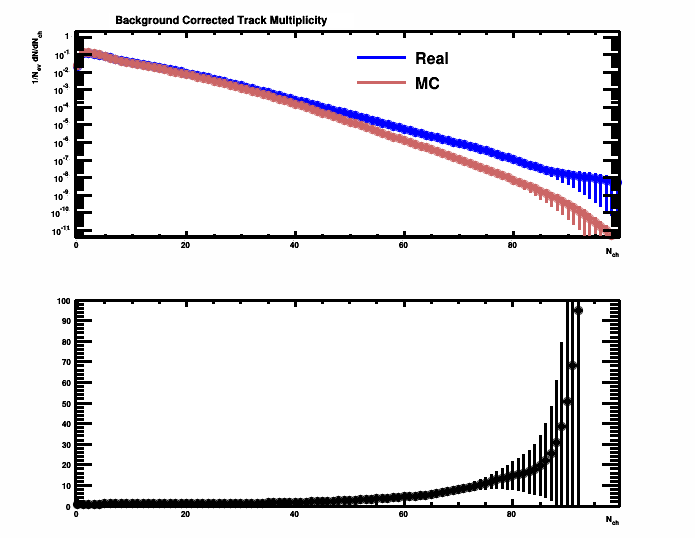
\includegraphics[width=\textwidth]{/afs/cern.ch/user/d/dvoong/cmtuser/DaVinci_v33r6/Phys/ChargedParticleMultiplicity/python/multiplicity/tracks/data_files/TrackMultiplicityPlottingJob/bk/Down/mc/-1/-1/bk/Down/mc/-1/-1/meissner_multiplicity_full/bk/Down/real/-1/-1/bk/Down/real/-1/-1/pngs/comparison/background_corrected/2-0_4-5_comparison.png}
%		\caption{$2.0 \le \eta \le 4.5$}
%	\end{subfigure}
%	\begin{subfigure}{0.32\textwidth}
%		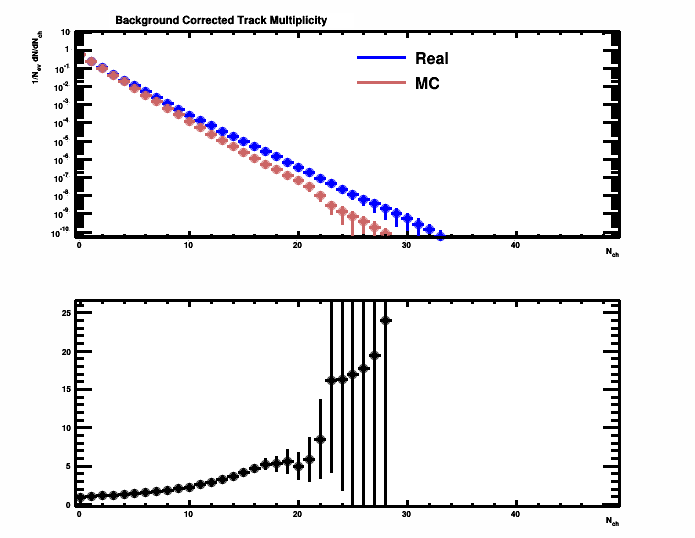
\includegraphics[width=\textwidth]{/afs/cern.ch/user/d/dvoong/cmtuser/DaVinci_v33r6/Phys/ChargedParticleMultiplicity/python/multiplicity/tracks/data_files/TrackMultiplicityPlottingJob/bk/Down/mc/-1/-1/bk/Down/mc/-1/-1/meissner_multiplicity/bk/Down/real/-1/-1/bk/Down/real/-1/-1/pngs/comparison/background_corrected/2-0_2-5_comparison.png}
%		\caption{$2.0 \le \eta \le 2.5$}
%	\end{subfigure}
%	\begin{subfigure}{0.32\textwidth}
%		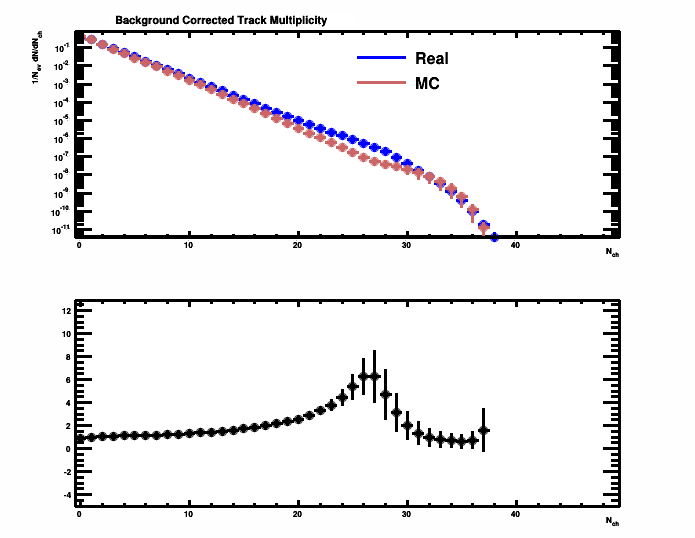
\includegraphics[width=\textwidth]{/afs/cern.ch/user/d/dvoong/cmtuser/DaVinci_v33r6/Phys/ChargedParticleMultiplicity/python/multiplicity/tracks/data_files/TrackMultiplicityPlottingJob/bk/Down/mc/-1/-1/bk/Down/mc/-1/-1/meissner_multiplicity/bk/Down/real/-1/-1/bk/Down/real/-1/-1/pngs/comparison/background_corrected/2-5_3-0_comparison.png}
%		\caption{$2.5 \le \eta \le 3.0$}
%	\end{subfigure}
%	\begin{subfigure}{0.32\textwidth}
%		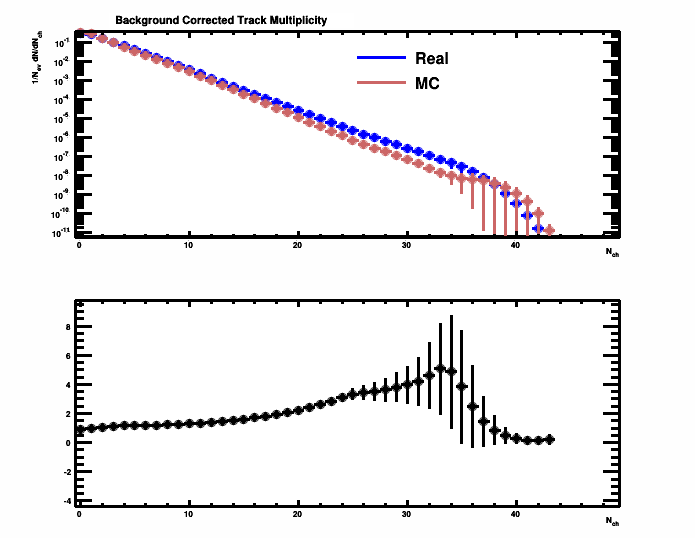
\includegraphics[width=\textwidth]{/afs/cern.ch/user/d/dvoong/cmtuser/DaVinci_v33r6/Phys/ChargedParticleMultiplicity/python/multiplicity/tracks/data_files/TrackMultiplicityPlottingJob/bk/Down/mc/-1/-1/bk/Down/mc/-1/-1/meissner_multiplicity/bk/Down/real/-1/-1/bk/Down/real/-1/-1/pngs/comparison/background_corrected/3-0_3-5_comparison.png}
%		\caption{$3.0 \le \eta \le 3.5$}
%	\end{subfigure}
%	\begin{subfigure}{0.32\textwidth}
%		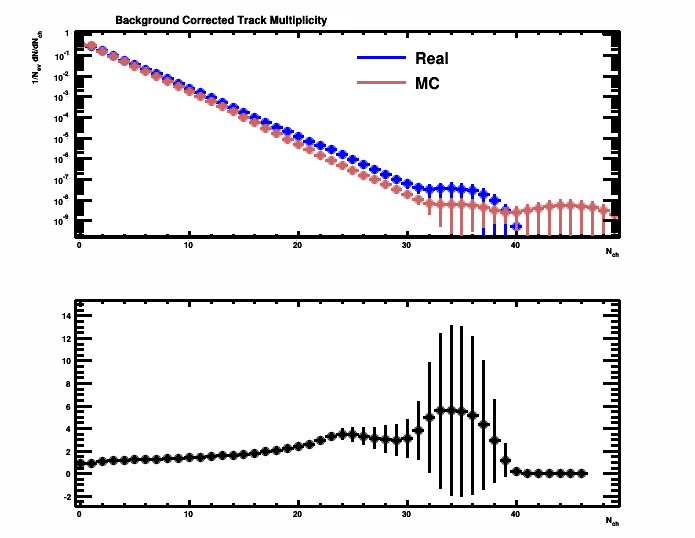
\includegraphics[width=\textwidth]{/afs/cern.ch/user/d/dvoong/cmtuser/DaVinci_v33r6/Phys/ChargedParticleMultiplicity/python/multiplicity/tracks/data_files/TrackMultiplicityPlottingJob/bk/Down/mc/-1/-1/bk/Down/mc/-1/-1/meissner_multiplicity/bk/Down/real/-1/-1/bk/Down/real/-1/-1/pngs/comparison/background_corrected/3-5_4-0_comparison.png}
%		\caption{$3.5 \le \eta \le 4.0$}
%	\end{subfigure}
%	\begin{subfigure}{0.32\textwidth}
%		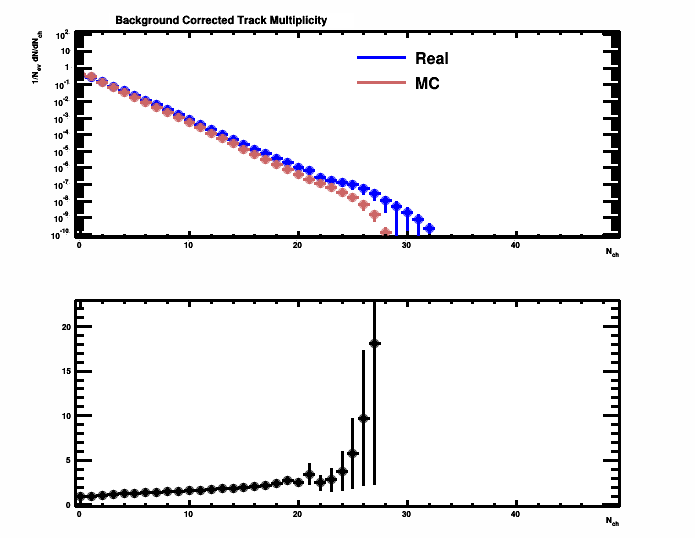
\includegraphics[width=\textwidth]{/afs/cern.ch/user/d/dvoong/cmtuser/DaVinci_v33r6/Phys/ChargedParticleMultiplicity/python/multiplicity/tracks/data_files/TrackMultiplicityPlottingJob/bk/Down/mc/-1/-1/bk/Down/mc/-1/-1/meissner_multiplicity/bk/Down/real/-1/-1/bk/Down/real/-1/-1/pngs/comparison/background_corrected/4-0_4-5_comparison.png}
%		\caption{$4.0 \le \eta \le 4.5$}
%	\end{subfigure}
%	\caption{Background corrected track multiplicities from real data and MC}
%	\label{fig: background corrected track multiplicity comparison}
%\end{figure}

\begin{figure}[H]
	\centering
	\begin{subfigure}{0.32\textwidth}
		\includegraphics[width=\textwidth]{Chapters/multiplicity/images/background_corrected/real/2-0_4-5_norm.png}
		\caption{$2.0 \le \eta \le 4.5$}
	\end{subfigure}
	\begin{subfigure}{0.32\textwidth}
		\includegraphics[width=\textwidth]{Chapters/multiplicity/images/background_corrected/real/2-0_2-5_norm.png}
		\caption{$2.0 \le \eta \le 2.5$}
	\end{subfigure}
	\begin{subfigure}{0.32\textwidth}
		\includegraphics[width=\textwidth]{Chapters/multiplicity/images/background_corrected/real/2-5_3-0_norm.png}
		\caption{$2.5 \le \eta \le 3.0$}
	\end{subfigure}
	\begin{subfigure}{0.32\textwidth}
		\includegraphics[width=\textwidth]{Chapters/multiplicity/images/background_corrected/real/3-0_3-5_norm.png}
		\caption{$3.0 \le \eta \le 3.5$}
	\end{subfigure}
	\begin{subfigure}{0.32\textwidth}
		\includegraphics[width=\textwidth]{Chapters/multiplicity/images/background_corrected/real/3-5_4-0_norm.png}
		\caption{$3.5 \le \eta \le 4.0$}
	\end{subfigure}
	\begin{subfigure}{0.32\textwidth}
		\includegraphics[width=\textwidth]{Chapters/multiplicity/images/background_corrected/real/4-0_4-5_norm.png}
		\caption{$4.0 \le \eta \le 4.5$}
	\end{subfigure}
	\caption{Background corrected track multiplicities in measured data}
	\label{fig: background corrected track multiplicities}
\end{figure}

\begin{figure}[H]
	\centering
	\begin{subfigure}{0.32\textwidth}
		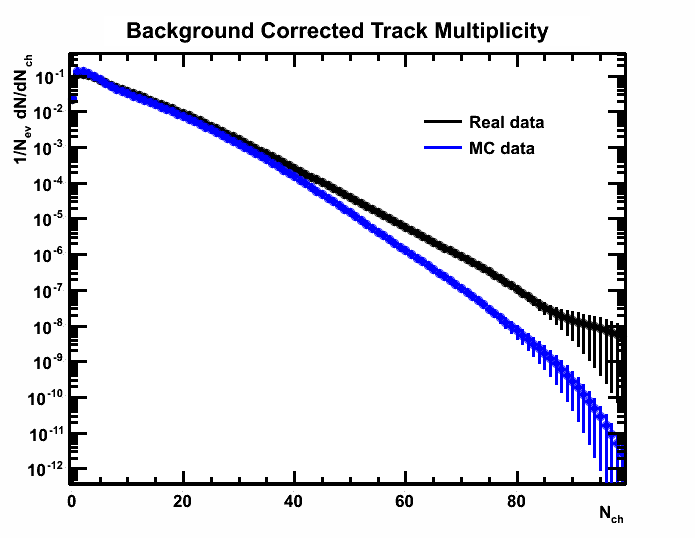
\includegraphics[width=\textwidth]{Chapters/multiplicity/charged_particle_event_multiplicity/images/background_correction_comparison/2_0-4_5.png}
		\caption{$2.0 \le \eta \le 4.5$}
	\end{subfigure}
	\begin{subfigure}{0.32\textwidth}
		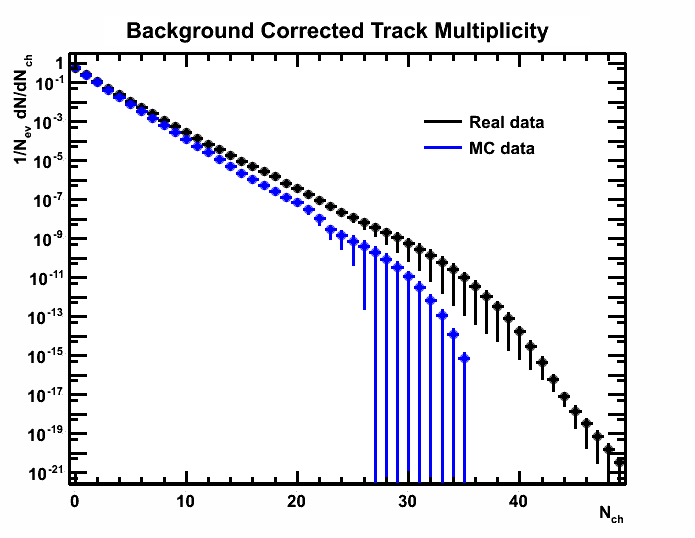
\includegraphics[width=\textwidth]{Chapters/multiplicity/charged_particle_event_multiplicity/images/background_correction_comparison/2_0-2_5.png}
		\caption{$2.0 \le \eta \le 2.5$}
	\end{subfigure}
	\begin{subfigure}{0.32\textwidth}
		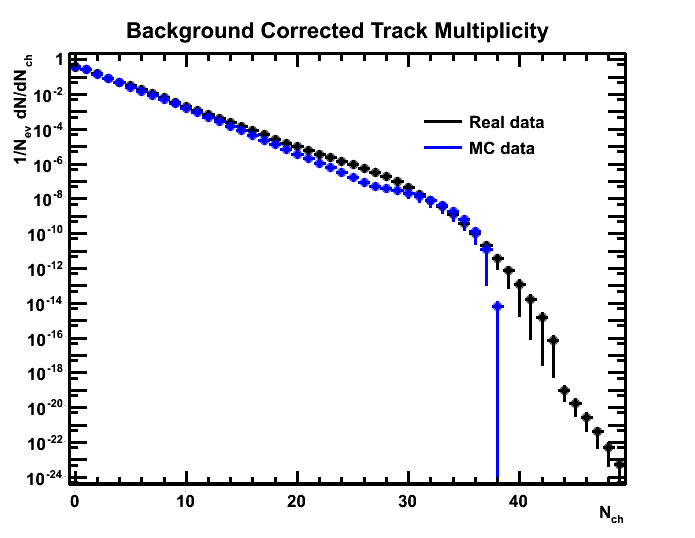
\includegraphics[width=\textwidth]{Chapters/multiplicity/charged_particle_event_multiplicity/images/background_correction_comparison/2_5-3_0.png}
		\caption{$2.5 \le \eta \le 3.0$}
	\end{subfigure}
	\begin{subfigure}{0.32\textwidth}
		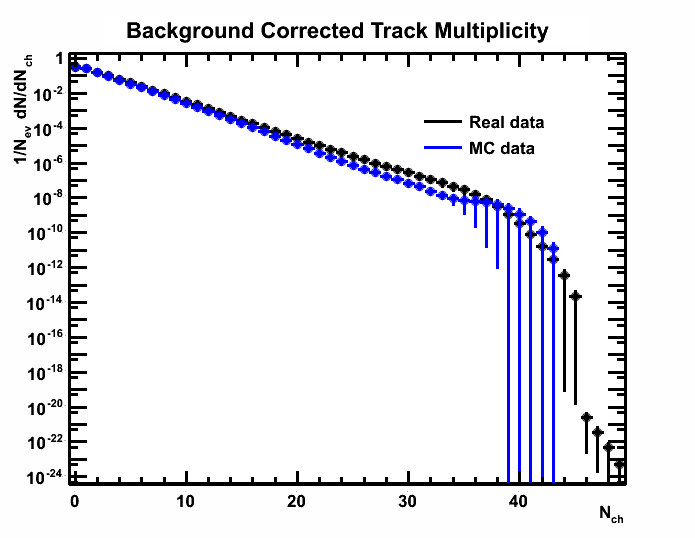
\includegraphics[width=\textwidth]{Chapters/multiplicity/charged_particle_event_multiplicity/images/background_correction_comparison/3_0-3_5.png}
		\caption{$3.0 \le \eta \le 3.5$}
	\end{subfigure}
	\begin{subfigure}{0.32\textwidth}
		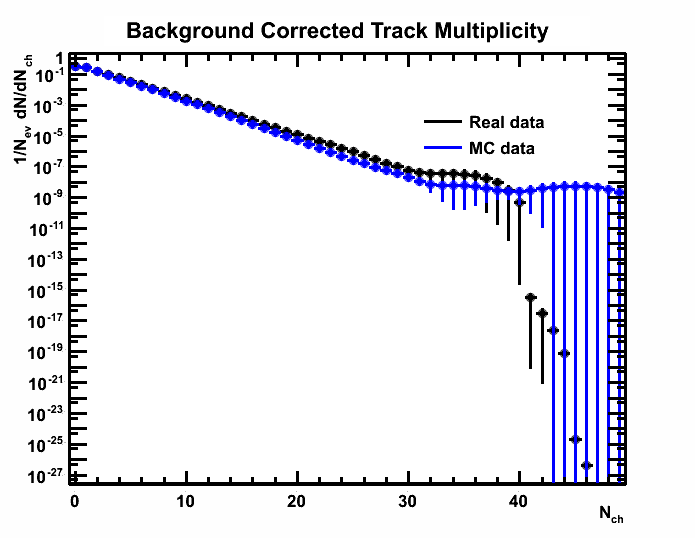
\includegraphics[width=\textwidth]{Chapters/multiplicity/charged_particle_event_multiplicity/images/background_correction_comparison/3_5-4_0.png}
		\caption{$3.5 \le \eta \le 4.0$}
	\end{subfigure}
	\begin{subfigure}{0.32\textwidth}
		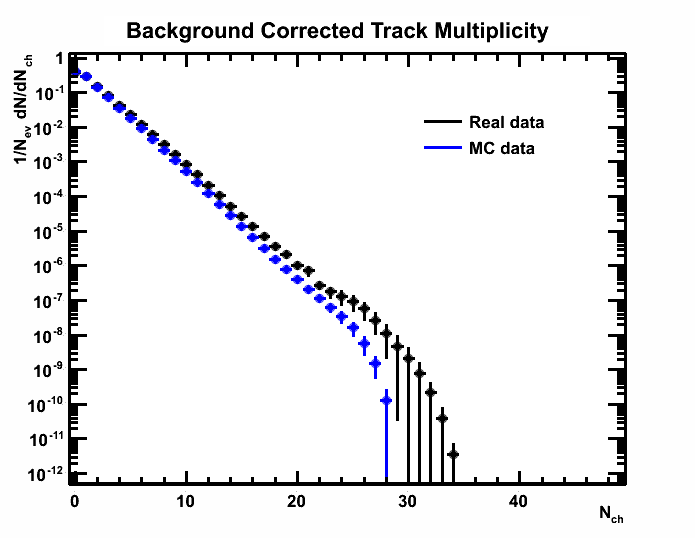
\includegraphics[width=\textwidth]{Chapters/multiplicity/charged_particle_event_multiplicity/images/background_correction_comparison/4_0-4_5.png}
		\caption{$4.0 \le \eta \le 4.5$}
	\end{subfigure}
	\caption{Background corrected track multiplicities from measured data and MC}
	\label{fig: background corrected track multiplicity comparison}
\end{figure}

%\begin{figure}[h]
%	\centering
%	\begin{subfigure}{0.32\textwidth}
%		\includegraphics[width=\textwidth]{/afs/cern.ch/user/d/dvoong/cmtuser/DaVinci_v33r6/Phys/ChargedParticleMultiplicity/python/multiplicity/tracks/data_files/TrackMultiplicityPlottingJob/bk/Down/mc/-1/-1/bk/Down/mc/-1/-1/meissner_multiplicity_full/bk/Down/mc/-1/-1/bk/Down/mc/-1/-1/pngs/cross_check/2-0_4-5.png}
%		\caption{$2.0 \le \eta \le 4.5$}
%	\end{subfigure}
%	\begin{subfigure}{0.32\textwidth}
%		\includegraphics[width=\textwidth]{/afs/cern.ch/user/d/dvoong/cmtuser/DaVinci_v33r6/Phys/ChargedParticleMultiplicity/python/multiplicity/tracks/data_files/TrackMultiplicityPlottingJob/bk/Down/mc/-1/-1/bk/Down/mc/-1/-1/meissner_multiplicity/bk/Down/mc/-1/-1/bk/Down/mc/-1/-1/pngs/cross_check/2-0_2-5.png}
%		\caption{$2.0 \le \eta \le 2.5$}
%	\end{subfigure}
%	\begin{subfigure}{0.32\textwidth}
%		\includegraphics[width=\textwidth]{/afs/cern.ch/user/d/dvoong/cmtuser/DaVinci_v33r6/Phys/ChargedParticleMultiplicity/python/multiplicity/tracks/data_files/TrackMultiplicityPlottingJob/bk/Down/mc/-1/-1/bk/Down/mc/-1/-1/meissner_multiplicity/bk/Down/mc/-1/-1/bk/Down/mc/-1/-1/pngs/cross_check/2-5_3-0.png}
%		\caption{$2.5 \le \eta \le 3.0$}
%	\end{subfigure}
%	\begin{subfigure}{0.32\textwidth}
%		\includegraphics[width=\textwidth]{/afs/cern.ch/user/d/dvoong/cmtuser/DaVinci_v33r6/Phys/ChargedParticleMultiplicity/python/multiplicity/tracks/data_files/TrackMultiplicityPlottingJob/bk/Down/mc/-1/-1/bk/Down/mc/-1/-1/meissner_multiplicity/bk/Down/mc/-1/-1/bk/Down/mc/-1/-1/pngs/cross_check/3-0_3-5.png}
%		\caption{$3.0 \le \eta \le 3.5$}
%	\end{subfigure}
%	\begin{subfigure}{0.32\textwidth}
%		\includegraphics[width=\textwidth]{/afs/cern.ch/user/d/dvoong/cmtuser/DaVinci_v33r6/Phys/ChargedParticleMultiplicity/python/multiplicity/tracks/data_files/TrackMultiplicityPlottingJob/bk/Down/mc/-1/-1/bk/Down/mc/-1/-1/meissner_multiplicity/bk/Down/mc/-1/-1/bk/Down/mc/-1/-1/pngs/cross_check/3-5_4-0.png}
%		\caption{$3.5 \le \eta \le 4.0$}
%	\end{subfigure}
%	\begin{subfigure}{0.32\textwidth}
%		\includegraphics[width=\textwidth]{/afs/cern.ch/user/d/dvoong/cmtuser/DaVinci_v33r6/Phys/ChargedParticleMultiplicity/python/multiplicity/tracks/data_files/TrackMultiplicityPlottingJob/bk/Down/mc/-1/-1/bk/Down/mc/-1/-1/meissner_multiplicity/bk/Down/mc/-1/-1/bk/Down/mc/-1/-1/pngs/cross_check/4-0_4-5.png}
%		\caption{$4.0 \le \eta \le 4.5$}
%	\end{subfigure}
%	\caption{Background correction cross-check. Background corrected track multiplicities are compared with tracks matched to generator prompt particles by MC truth matching}
%	\label{fig: background corrected track multiplicity cross-check}
%\end{figure}